\documentclass[12pt,a4]{article}
\pagestyle{plain}                           
\setlength{\textwidth}{6.5in}     
\setlength{\oddsidemargin}{0in} 
\setlength{\evensidemargin}{0in}  
\setlength{\textheight}{8.5in}   
\setlength{\topmargin}{0in}      
\setlength{\headheight}{0in}      
\setlength{\headsep}{0in}    
\setlength{\footskip}{0.5in}    

%these packages produce nice-looking math, with extra symbols and formatting
\usepackage{graphicx}
\usepackage{mathrsfs}
\usepackage{color}
\usepackage{epsfig}
\usepackage{epstopdf}
\usepackage{epsf}
\usepackage{url}
\usepackage{setspace}
\usepackage[colorlinks=true,urlcolor=blue]{hyperref}
\usepackage{amsmath,amsthm,amsfonts,amssymb}
\usepackage{tocloft}
\usepackage{multirow}
\usepackage{floatflt}
\usepackage[wide]{sidecap}
\usepackage{paralist}
\usepackage{float}
\usepackage{hanging}
\linespread{1.05}


%%%%%%%%%%%%%%%%%%%%%%%%%%
\theoremstyle{plain} %soley's environments for theorems
\newtheorem{prop}{Proposition}[section]
\newtheorem{cond}[prop]{Condition}
\newtheorem{Def}{Definition}[section]
\newtheorem{theorem}{Theorem}[section]
\newtheorem{lemma}{Lemma}[section]
\newtheorem{ex}[prop]{Example}
%%%%%%%%%%%%%%%%%%%%%%%%%%


\newcommand{\ds}{\displaystyle}   % this command makes equations look nicer

\renewcommand{\thesubsection}{\thesection.\alph{subsection}}

\begin{document}

\author{Hugh McCreery, Johnathan Castillo}
\title{Kriging with Atmospheric Mercury Concentrations}
\maketitle

\noindent \textbf{\Large Abstract} \\
This paper attempted to examine the issue of mercury pollution by using spatial methods to predict the levels of three different types of pollutants at locations primarily in the Eastern United States. Using data from the National Atmospheric Deposition Program, we attempted to use both empirical variograms as well as maximum likelihood methods to estimate the covariance structure for each type of pollutant. After maximum likelihood analysis, we decided to use the estimated covariance structure from one type of pollutant for all pollutants as the other structures did not have logical physical interpretations. We then used simple kriging to generate predictions at locations without values. The usefulness of these predictions were hampered by the lack of input data and the input data being potentially non-stationary, and as a result we weren't able to confidently draw conclusions.

\newpage
{
\hypersetup{linkcolor = black}
\tableofcontents
}
\newpage

\section{Introduction}

In this paper, we worked with a data set from the National Atmospheric Deposition Program describing mercury pollution levels primarily centered around the eastern United States. We decided to use this data as the rising levels of pollution is a critical issue facing the world today. This mercury pollution, created primarily from coal mining and small-scale gold mining, can cause irreversible toxic effects to both the health of humans and the ecosystems around us (Ankrah). These potential harms of mercury and the resulting desire to monitor the levels of their pollution lead us to attempt to find potential sources of pollution. We hope to use the observed data of the mercury concentrations at different atmospheric locations to estimate the mercury concentration at locations without known values across the eastern United States. If we are able to create meaningful predictions of the pollution levels, we also wanted to consider if these predictions could be used to determine the possible sources of the pollution.

The data set contains information about three different types of mercury pollution - Particulate Bound Mercury (PBM), Gaseous Oxidized Mercury (GOM), and Gaseous Elemental Mercury (GEM). The data spans from 2008 to 2018, but as we didn't want to consider time in our analysis, we took the average amounts of each pollution for each station from 2015-2017 and used those as the values to be considered. In addition, we didn't consider stations that were very far away from the rest of our data (such as one in Taiwan) and any data marked as ``invalid" in the metadata. This left us with 21 stations with valid data for each of the three types of pollution, as shown in the plots below.

\begin{figure}[H]
    \centering
    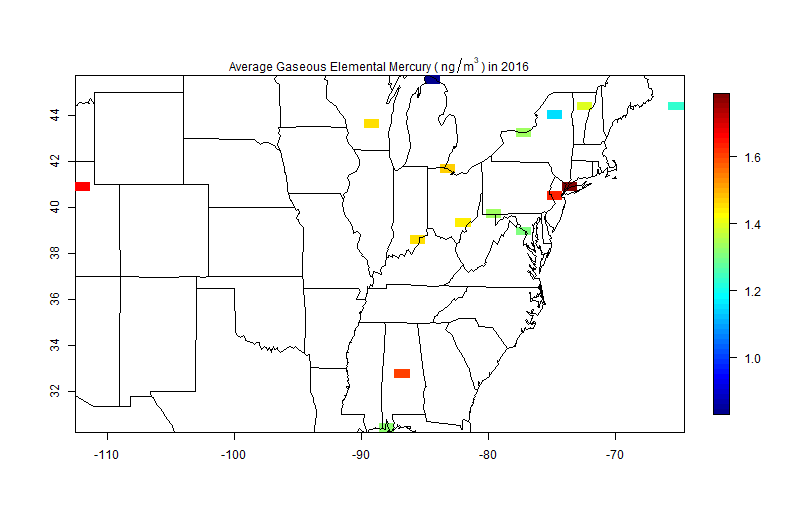
\includegraphics[width=0.65\linewidth]{GEM.png}
    \caption{Levels of Gaseous Elemental Mercury at each of the 21 valid measuing stations}
\end{figure}

\begin{figure}[H]
    \centering
    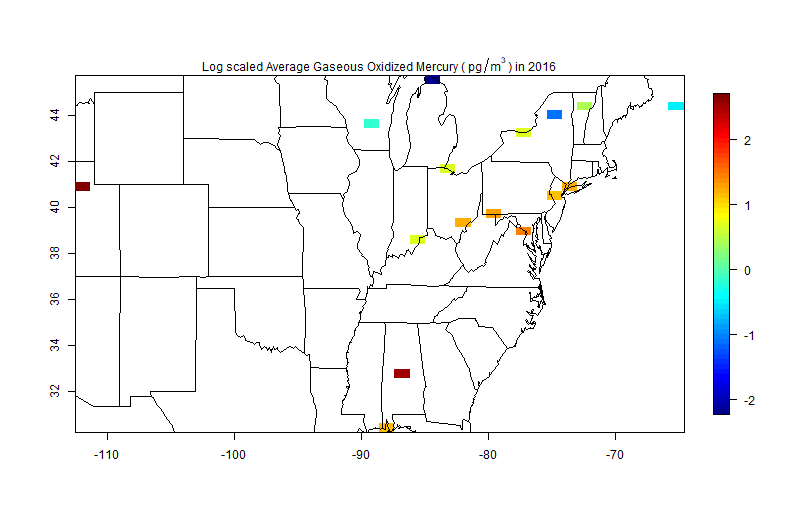
\includegraphics[width=0.65\linewidth]{GOM.png}
    \caption{Levels of log-scaled Gaseous Oxidized Mercury at each of the 21 valid measuing stations}
\end{figure}

\begin{figure}[H]
    \centering
    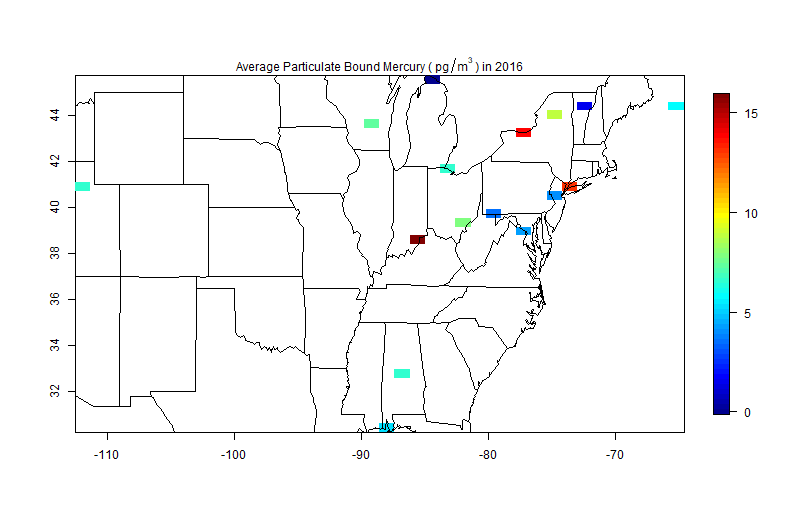
\includegraphics[width=0.65\linewidth]{PBM.png}
    \caption{Levels of Particulate Bound Mercury at each of the 21 valid measuring stations}
\end{figure}

\section{Methods and Results}
To start our analysis, we first obtained the mercury data from the NADP and imported the data into R (``AMNet..."). Then, using the provided information about each site, we matched each station from the initial data file with its geographic location. Invalid data was then removed based on the metadata descriptions. \\
After plotting the mercury data for each station, the data was partitioned into 3 areas with roughly the same number of stations. The means of the mercury concentrations in each partition were calculated and compared to each other to test for stationarity. It was found that the GEM concentrations appeared to be relatively stationary, while the GOM and PBM concentrations appeared to be potentially non-stationary. To simplify further analysis, we've decided to assume stationarity for each of the mercury concentrations despite the potentially non-stationary nature of the data. \\
Empirical variograms were also calculated for each mercury concentration using the \textbf{variog} function from the \textbf{geoR} package in R and have been included below.
\begin{figure}[H]
    \centering
    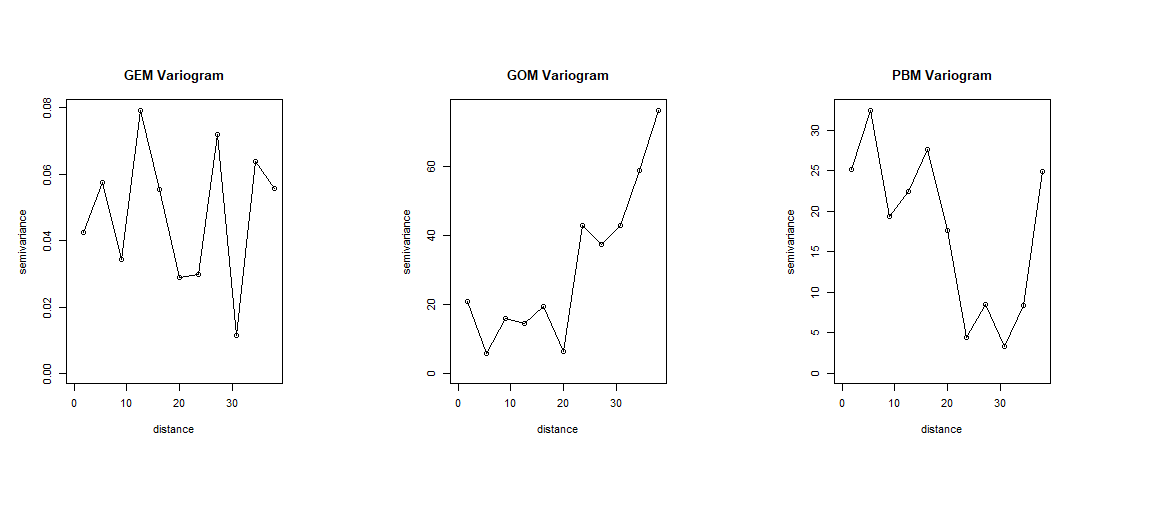
\includegraphics[width=\linewidth]{merc_variograms.png}
    \caption{Empirical Variograms for GEM, GOM, and PBM concentrations based on the observed data.}
\end{figure}
Unfortunately, the small sample size of the data resulted in only a few points at most for each distance (lag), and so our empirical variogram calculations were not useful. This meant we needed to use the maximum likelihood estimation approach to estimate the covariance structures for the mercury concentrations. \\
For maximum likelihood estimation, we first assumed that each of the concentrations would have a exponential covariance structure. We felt confident making this assumption because exponential covariance structures are common in climate modeling. A possible nugget term was also included, giving us a total of 3 spatial parameters to estimate: $\tau^2$ (nugget variance), $\sigma^2$ (process variance), and $\lambda$ (range parameter of exponential covariance). Additionally, since it appeared the concentrations did not have a mean centered at 0, the data sets were detrended. \\
Maximum likelihood estimation of ($\tau, \sigma^2, \lambda$) using the negative log likelihood was done using both a 3-dimensional grid search and R's built in \textbf{optim} function. Using the grid search method, it was found that for the GOM concentrations the MLE estimates were: 
\begin{center}
($\hat{\tau},\hat{\sigma}^2,\hat{\lambda}$) = (0, 0.4081, 234.7) 
\end{center}
with similar results using the \textbf{optim} function. \\
An important note is that the station located in Utah seemed too far away from the rest of the observations and thus was not used in the rest of our analysis. The station being very far from the rest of the points was distorting the parameter values. Initially, we believed that this point was close enough spatially to the rest of our data but got better results not using it. The results of our grid search have been visualized below.
\begin{figure}[H]
    \centering
    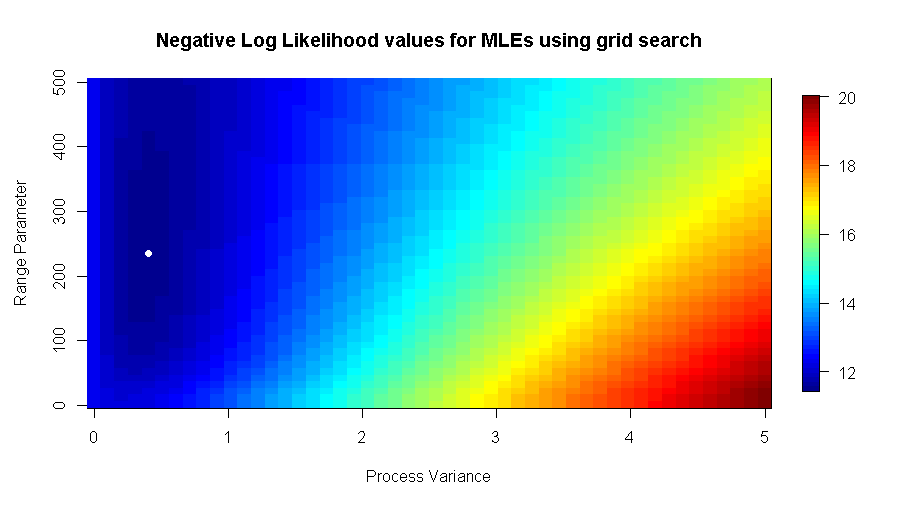
\includegraphics[width=0.7\linewidth]{GOM_gridsearch.png}
    \caption{Negative log-likelihood values for MLE estimation of GOM covariance parameters $\hat{\sigma}^2$ and $\hat{\lambda}$ ($\hat{\tau}$ not shown since estimate was 0). The white dot indicates where the negative log-likelihood is minimized.}
\end{figure}
Having determined the covariance structure for the GOM data, we then attempted to find the MLEs for the covariance structure of the PBM and GEM using the same process. However, we ran into issues where the resulting estimates had interpretations that weren't logical. For the GEM data, the MLE for $\sigma^2$ was 0, indicating the data had no spatial correlation. Similarly, when we created MLEs for the PBM data, we found that the estimate for the range parameter was extremely small, which lead the kriged values to equal the mean at almost every point. As neither of these estimates gave useful results, we chose to assume that each of the types of mercury pollution would have similar covariance structures and used the parameter estimates from the GOM data to krige the PBM and GEM data. \\
Using these MLE estimates for the covariance structure, the concentrations at unobserved locations were predicted using simple kriging methods.
\begin{figure}[H]
    \centering
    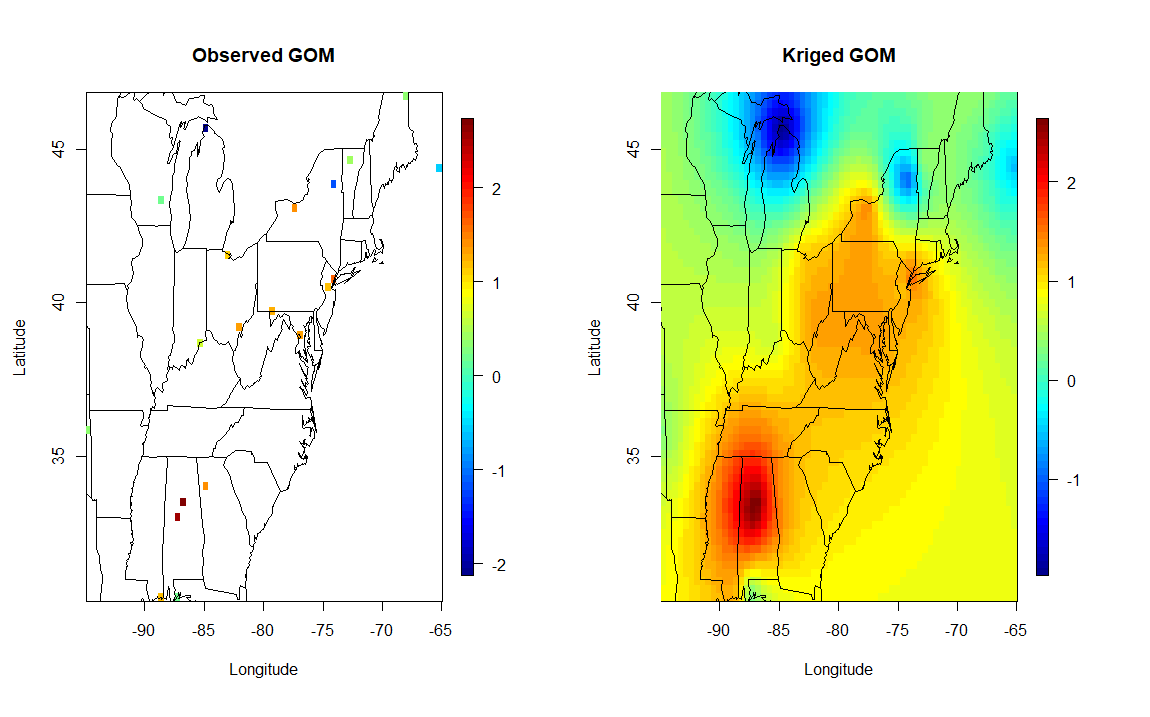
\includegraphics[width=0.7\linewidth]{krig_GOM.png}
    \caption{Observed GOM concentrations and Kriged GOM concentrations}
\end{figure}
\begin{figure}[H]
    \centering
    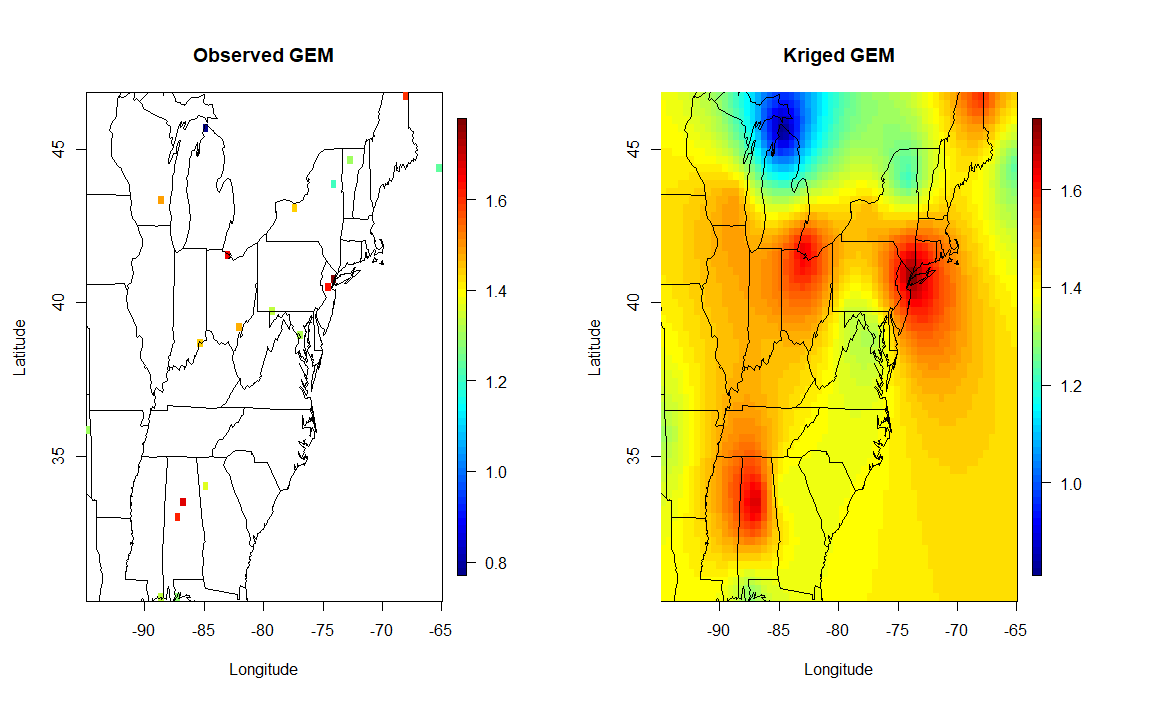
\includegraphics[width=0.7\linewidth]{krig_GEM.png}
    \caption{Observed GEM concentrations and Kriged GEM concentrations}
\end{figure}
\begin{figure}[H]
    \centering
    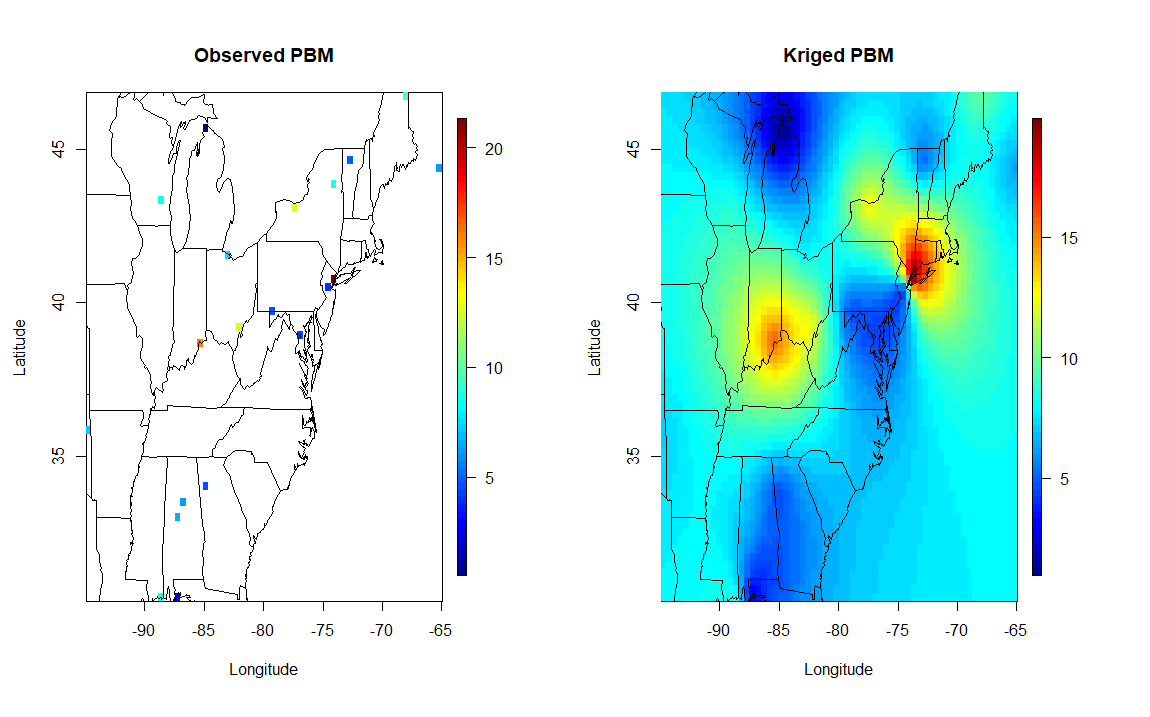
\includegraphics[width=0.7\linewidth]{krig_PBM.png}
    \caption{Observed PBM concentrations and Kriged PBM concentrations}
\end{figure}
Kriging uncertainties were also calculated for the kriging estimates. Since each type of concentration were assumed to have the same covariance model, the kriging uncertainties for each concentration are the same.
\begin{figure}[H]
    \centering
    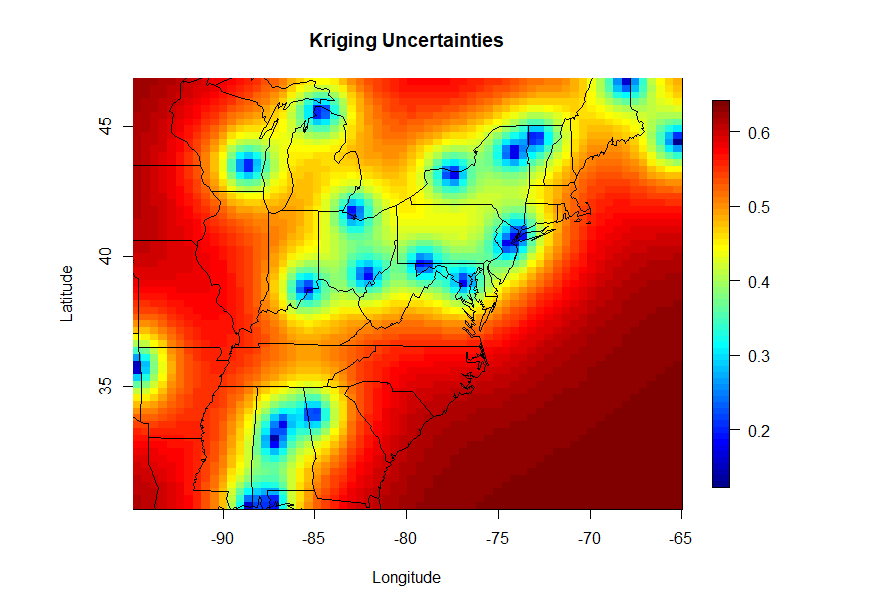
\includegraphics[width=0.7\linewidth]{krig_uncert.png}
    \caption{Simple Kriging uncertainties based on location. Due to the small sample size, our uncertainties are quite high in many areas of the map.}
\end{figure}

\section{Implications and Analysis}


Overall, our lack of data hampered our ability to draw any strong conclusions from our analysis and generate the accurate predictions we desired.  The empirical variograms we calculated didn't lead us to believe that we would be able to determine a spatial correlation through that method and the estimates of parameters using MLEs had large variances. Additionally, our MLE estimates relied on assuming all three types of pollution had the same covariance structure, which is likely incorrect. Therefore, while we did get some results, they were hindered by their large uncertainties and as a result didn't give very useful information. This also resulted in us not being able to use our analysis to predict any outside sources of pollution. Our kriged estimates mainly capture the hot and cold spots of the observed locations which limits our ability to identify any potentially high pollution areas outside of observations.

Finally, our assumption that the data is stationary for each of the types of pollution may not necessarily hold. When we tested for stationarity, our results indicated that the GOM and PBM concentrations may not be stationary. While we performed our analysis under the assumption of stationarity anyway, it represents a significant weakness in our analysis that we weren't certain that the processes were stationary.


\section{Further Research}
If we were to continue research on this topic, the most important improvement we would make would be to find a more complete data set. The fact that we had very few data points limited our ability to draw any strong conclusions. Using the same analysis that we completed earlier on a larger data set would greatly improve many of our issues determining stationarity and the large uncertainties associated with the MLEs and kriged values.

Additionally, we could attempt to use non-stationary techniques to analyze our data. As noted earlier, while it appeared the GEM data was stationary, the GOM and PBM data looked to be potentially non-stationary. If we don't use this assumption of stationarity, our potential results may be more accurate.

Finally, we might attempt find possible covariates for our data to help improve our predictions. As noted earlier, the major causes of mercury pollution come from coal and gold mining, so finding data relating to where these industries operate could be useful as covariates in future analysis. We may also find other types of pollution (such as air pollution from coal burning) useful as well.

\newpage

\section{References}
\begin{hangparas}{.25in}{1}
    ``AMNet Data Retrieval" \textit{National Atmospheric Deposition Program}. 2018.\\ http://nadp.slh.wisc.edu/data/AMNet/. 8 Dec 2018. \\
    
    Ankrah, Rodges. ``Mercury Emissions: The Global Context." \textit{United States Environmental Protection Agency}. 21 Nov 2018. https://www.epa.gov/international-cooperation/mercury-emissions-global-context. 8 Dec 2018.
\end{hangparas}
\end{document}
